% Chapter 4

\chapter{Autonomic Cloud Computing SLA Management Approach} % Main chapter title
\label{ASLAMaaSApproach} % For referencing the chapter elsewhere, use \ref{Chapter1} 

\section{Autonomic Computing}
The ever increasing complexity, multi dimensionality and abstraction of modern computer systems make it difficult for users to utilize, maintain and fully understand them. With this issue in mind, IBM \cite{horn2001autonomic} developed a concept for autonomous systems and coined the phrase Autonomic Computing. According to the IBM’s vision autonomic behaviour can be characterised by key capabilities such as self-diagnosis, self-configuration, self-adaption and self-healing, which are all focusing on the continuous executability of a computer system without the need of user interaction. There are sveral definitions for autonomic computing, following the most common ones are stated:

\begin{itemize} 
\item ''The vision of autonomic computing is to create software through self-* properties'' \cite{sterritt2005autonomic}.
\item ''Autonomic computing is the ability to manage your computing enterprise
through hardware and software that automatically and dynamically responds to the
requirements of your business'' \cite{murch2004autonomic}.
\item ''Autonomic computing is the ability to manage your computing enterprise
through hardware and software that automatically and dynamically responds to the
requirements of your business'' \cite{murch2004autonomic}.
\end{itemize} 

The phrase autonomic is derived from human biology, where the autonomic nervous system keeps track of the bodies vital functions such as heartbeat, temperature and breathing  while working in the background. However, there are main differences between the human body and autonomic systems. Firstly most of the tasks of the autonomic nervous system can't be controlled, where as the tasks of an autonomic systems are based on human written policies.
To make these policies work the system has the need for sensing the state of the system and its enviornment. According to the IBM vison, a autonomic system consists many interacting autonomic elements. These elements control the autonomic computing environment, consisting of other autonomic elements or the managed system, based on defined policies. This was modeled into the autonomic control loop (MAPE-K paradigm).

\begin{figure}[ht]
\begin{center}
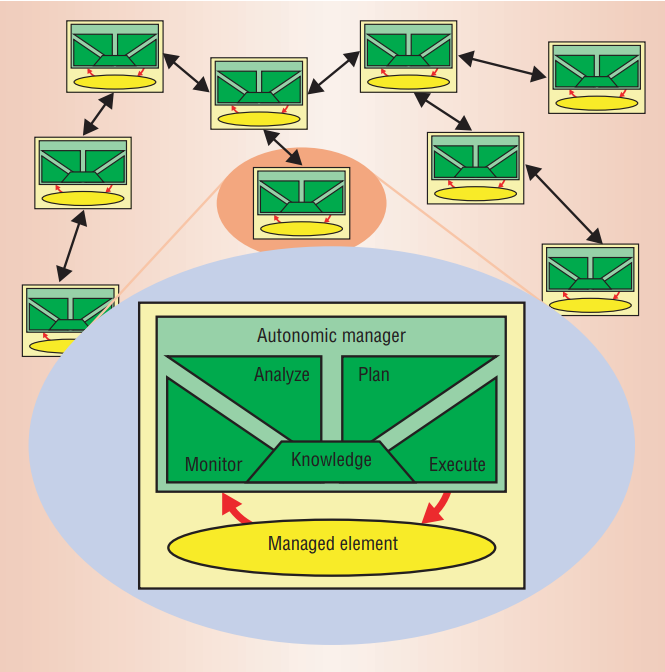
\includegraphics[width=0.5\textwidth]{chapters/chapter4/fig/mape2.png}
\end{center}
\caption{Autonomic Control Loop (MAPE-K) after \cite{kephart2003vision}}
\label{fig:SLA_Structure}
\end{figure}

The four phases, monitoring, analysis, planning and execution are extendend by a common knowledge base and form the so called autonomic manager, which directly interacts with the managed element. Such managed elements can consists of, for example CPU, network nodes, virtual machine instances, databases or applications. 

\begin{itemize} 
\item \textbf{Monitoring} is collecting informations and metadata about the status, process and trend of the managed element. Here 
various methods of monitoring can be used, such as push or pull systems or agent-based systems to periodically retrive the needed information.  
\item \textbf{Analysis} uses these collected informations to decide whether or not the indicaton of an event to start an adaptation action has been reached. If such an event occurs an action strategy should be created to adapt and adjust the system to the targeted state.
\item \textbf{Planning} uses this action strategy to create an adaption plan based on the targeted state and the current state of the system. This plan consists of instructions, wich in detail describe the actual changes and actions.
\item \textbf{Execution} runs these adaptations and adjustments. Herefore the execution of the system is altered and the adjustments are made. Afterwards the loop starts again.
\end{itemize} 

The Dynaco adaptation model proposes a similar approach to the MAPE for distributed application by leveraging component-based design \citep{buisson2005dynamic} \citep{buisson2006adaptation}. Autonomic computing aims to faciliate self-management of complex systems consistiong of various components. Autonomic computing systems involve service-oriented technologies, agent technologies, adaptive control theory, machinelearning, optimization theory, and many more \citep{fei2005design} \citep{zhao2009survey}. 
 
The aim of introducing this paradigm in this thesis, is to achieve autonomic behaviour in our proposed Cloud management infrastructure, whereby appropriate actions are taken towards the enforcement of SLAs and performance metrics.

This report has identified the requirement for cloud computing infrastructures to guarantee service qualities and the need for new mechanisms for the integration and management of service level agreements. 

%Weitere Probleme und Motivation % % % % % % % % % % % % % % %

However, to address the identified problems within the current cloud computing landscape a system is needed which supports dynamic and fine grained quality assurance, while being flexible enough to cope with the frequently changing infrastructure. And automation of the underlying SLA management process, which includes creation,  monitoring, reporting, control and adaption. Especially for this more research in the area of behavior analysis, prediction and anomaly detection is necessary.

\section{Autonomic SLA Management Architecture}
To empower cloud users with the possibility of  managed cloud service quality and simultaneously increase the trust, reliability and appear of cloud computing for business use, this research proposes the concept of autonomic continuous dynamic SLA management for clouds, which will be realized by the “Autonomic SLA Management as a Service (ASLAMaaS)” architecture. It is build upon the IBM developed autonomic manager concept MAPE-K \cite{MAPE-K} (Monitor-Analysis-Plan-Execute-Knowledge).

\begin{figure}[!ht]
\centering
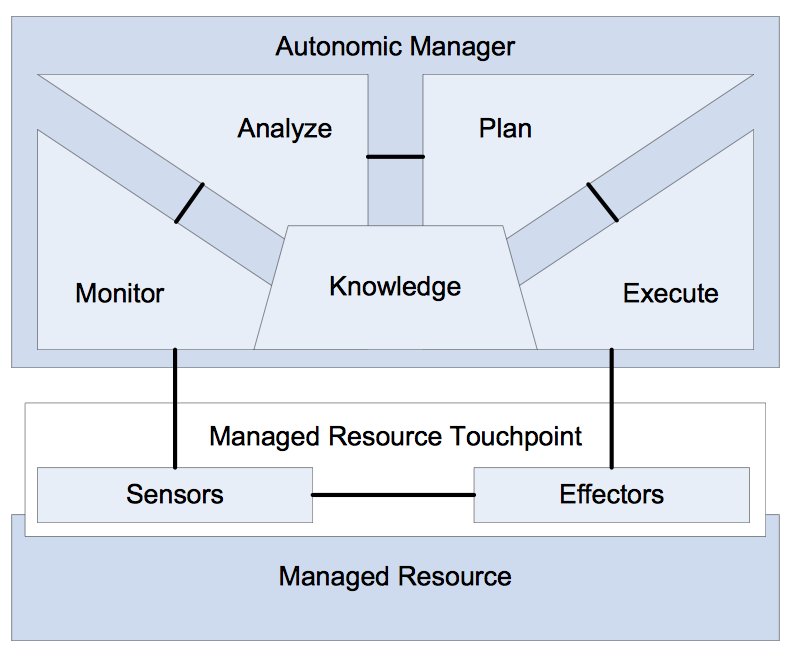
\includegraphics[width=3in]{chapters/chapter4/fig/MAPE.PNG}
\caption{Autonomic Computing Control Loop from \cite{MAPE-K}}
\label{fig_MAPE}
\end{figure}

%Agenten
%Monitoring
%Autonome Regelkreise
% Prediction

During the first phase of the research, cloud specific issues regarding the quality of cloud services and the need for dynamic management of service qualities were identified and analyzed, see Chapter 4. The ASLAMaaS framework is targeted on the following cloud challenges:

% %
% %
% %    Hier genau auflistung der Probleme wie keine Service garantien, schlechte Transparenz, herkömmliche verfahren zu langsam
% %
% %
The goals of the presented ASLAMaaS architecture are to integrate dynamic, autonomous SLA management into existing cloud infrastructures to enable cloud users to independently conclude SLAs for cloud services on a self service basis to improve the overall service quality and reliability, as well as increase the trust and economic use of cloud computing in general. For this the architecture shall enable continuous and flexible monitoring for cloud resources in regard of the corresponding service levels. Additionally advanced reporting and logging is integrated in every module of the architecture to enhance transparency between service provider and consumer by enabling comprehensibility.

Due to the strong dynamic and rapidly changing character of cloud computing, it is necessary that the system continuously adapts. Automomic computing systems are capable of continuous self-monitoring and adjustment. For this reason, the proposed architecture is based on autonomous modules which operate according to the principle MAPE-K. The overview of the components is shown in Figure \ref{fig_MAPE}.

\begin{figure}[!ht]
\centering
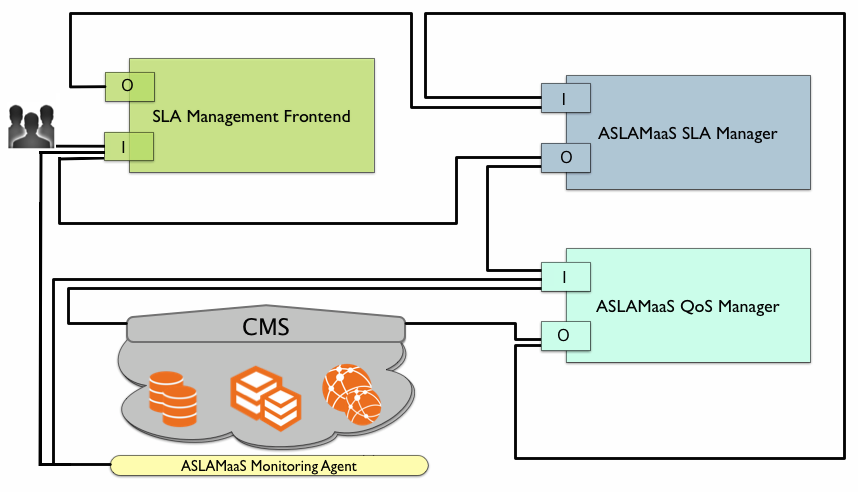
\includegraphics[width=4in]{chapters/chapter4/fig/ASLAMaaS3.PNG}
\caption{Information Flow between ASLAMaaS Modules}
\label{fig_Modules}
\end{figure}


For the monitoring of the autonomic system, a sensor is connected to the managed resource touch point, there the monitoring unit collects the data from the sensors and hands it over to the analysis unit, which then with the help of an external knowledge base creates action plans. These plans are carried out by the implementation unit (Execute), which adjusts the managed resource through effectors. In the case of a cloud infrastructure this could be upscaling the amount of CPUs of a VM instance.

The presented architecture consists of three main modules, the SLA Management Frontend, SLA Manager and the QoS Manager. The information flow between the individual modules can be seen in Figure \ref{fig_Modules}. The SLA Management Frontend thereby marks the input layer of the system, where users can create, monitor and adjust SLAs for their services.\\

\begin{figure}[!ht]
\centering
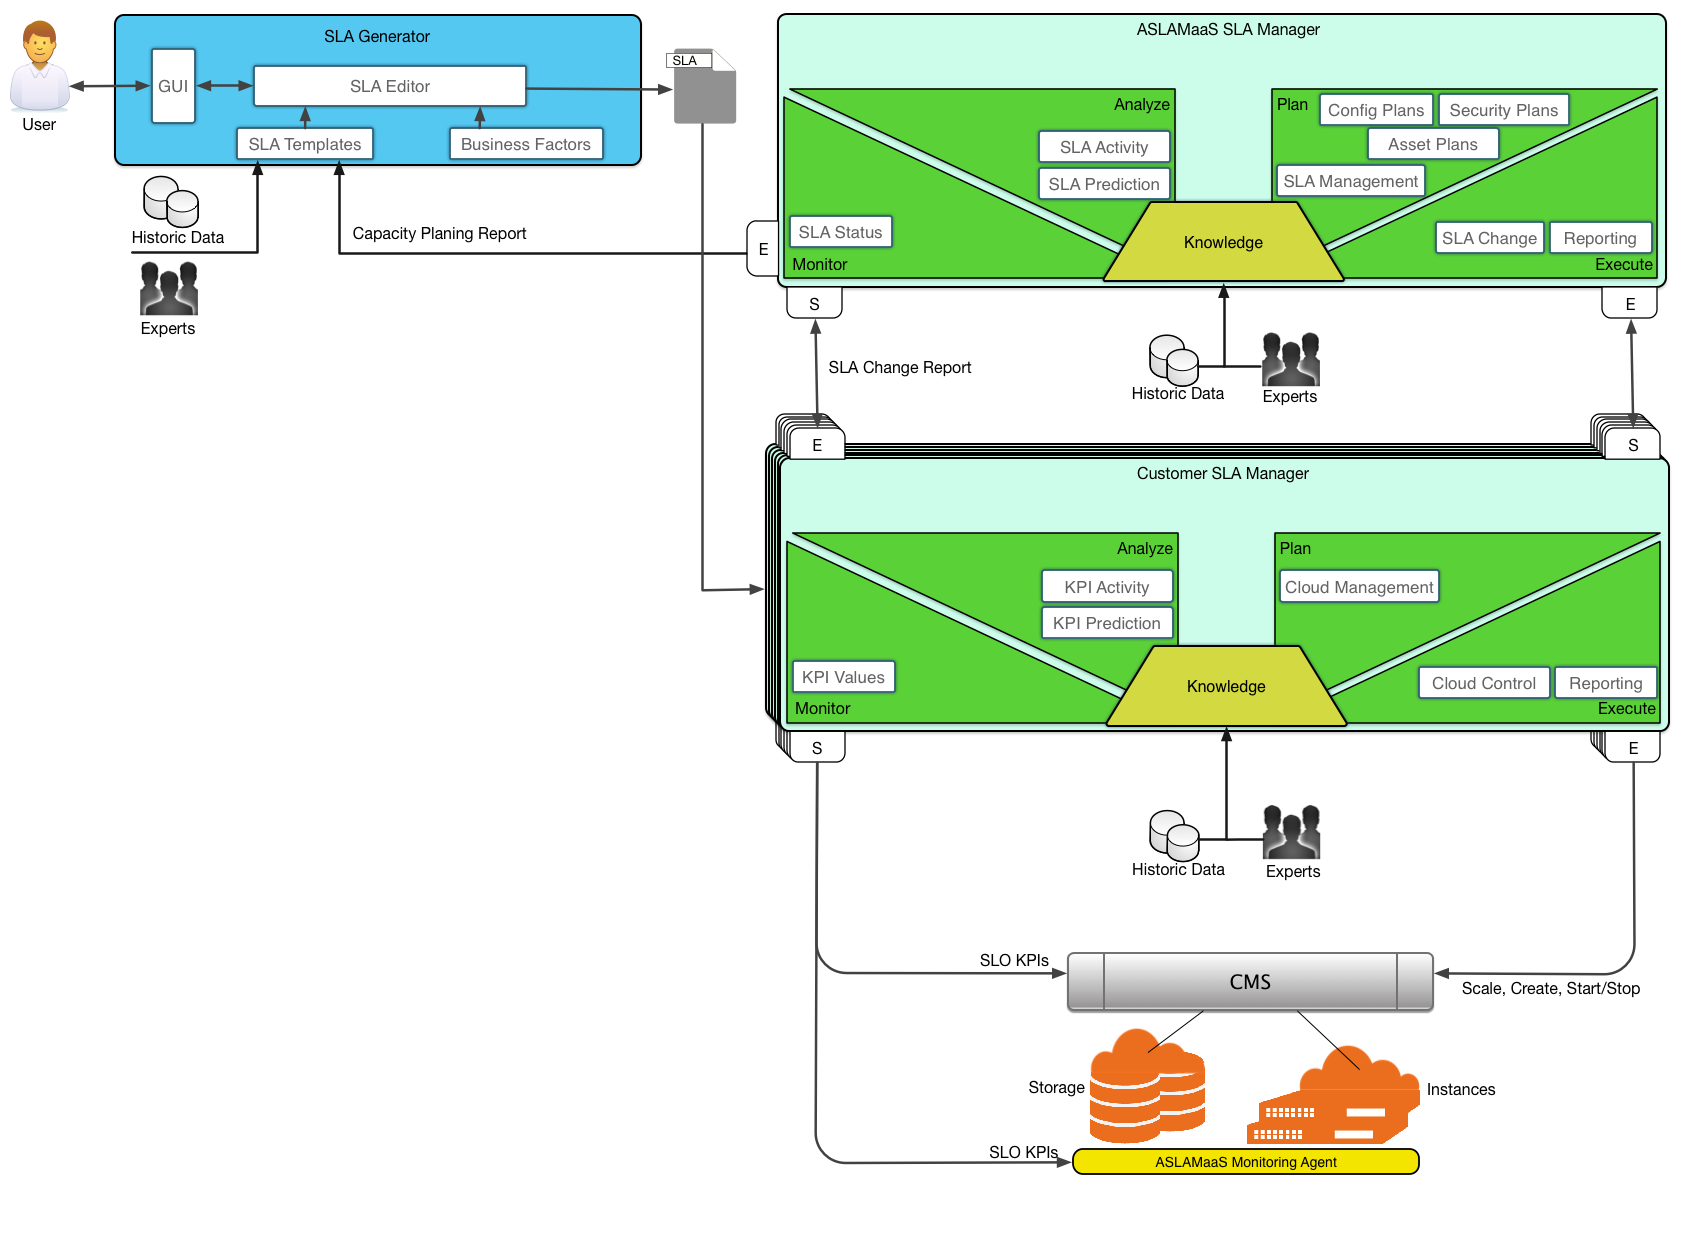
\includegraphics[width=5.3in]{chapters/chapter4/fig/ASLAMaaSArch.PNG}
\caption{ASLAMaaS Architecture Overview }
\label{fig_ASLAMaaSArch}
\end{figure}

To facilitate the process of creating new SLAs there will be a repository of pre-made SLA templates available within an graphical SLA editor. Thus users can easier and faster create their own specific SLAs by selecting a fitting template, which shall reflect best-practice and experience data for generalized types of services such as web services, databases systems, ERP systems and so on. The used SLA templates will use different key performance idicators (KPIs) grouped into categories based on their usage type. For each KPIs a specific QoS parameter and the associated metric has to be stored within the repository. A more detailed outlook on the SLA creation process and its components can be found in subsequent Chapter \ref{SLA creation}.


After the creation and activation of a  SLA for a cloud services the SLA Manager stores it in a repository and starts the autonomous control loop. An overview of the ASLAMaaS SLA Manager and its components is shown in Figure \ref{fig_SLAManager}. The SLA Manager is used as an abstraction level, in which the individual SLAs and their dependencies between each other are processed. Within the SLA Manager the general functionality regarding SLA compliance is processed. 

\begin{figure}[!ht]
\centering
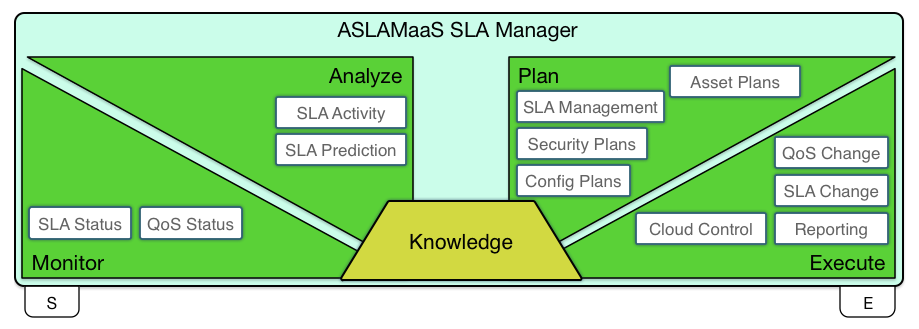
\includegraphics[width=5.3in]{chapters/chapter4/fig/SLAMan.PNG}
\caption{ASLAMaaS SLA Manager MAPE-K Loop }
\label{fig_SLAManager}
\end{figure}

For this measuring and keeping track of the status of each SLA and the containing service levels is needed. Therefore, the cloud management system,  virtual resources through intelligent agents and archived data will be used as input sources. Within the Analyze part the data is used to perceive the current state and predict the future behavior of the managed SLAs. Here the mutual influencing SLAs factors and the strategic business planing of the provider shall be weighed against each other. This could mean, for example, that in a state of emergency some contracts could be abandoned in favor of others so that the resulting financial damage will be reduced. Likewise here the beginning, suspension and stop of the dynamic SLAs and the total infrastructure overview data shall be used for strategic planing and pricing.  

Depending on the specific service, cloud SLAs may consist of several independent or conditional KPIs In order to ensure the service quality and operate within the agreed on limitations every KPI has to be controlled and monitored individually. For this every managed service level respectively KPI within a SLA will get its independent autonomous management loop. The corresponding graphical overview is shown in Figure \ref{fig_QoSManager} below.

\begin{figure}[!ht]
\centering
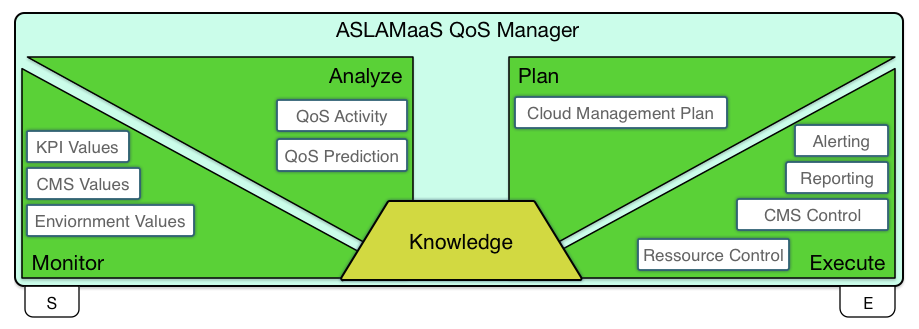
\includegraphics[width=5.3in]{chapters/chapter4/fig/QoSMan.PNG}
\caption{ASLAMaaS QoS Manager MAPE-K Loop }
\label{fig_QoSManager}
\end{figure}

The basic functionality will be nearly the same as the administration by the SLA Manager, only that instead of SLAs the individual QoS characteristics are directly influenced by adjustment of the cloud infrastructure and resources. So every SLA Manager instance will have multiple instances of the QoS Manager wich will take control of the corresponding parameters, monitoring and reporting. Starting by the Monitor, KPI relevant technical parameters, environmental data and dependencies are collected. This will be done by using the stored metrics for each KPI, deposited within the Knowledgebase. Such metrics will be measured either directly within the Cloud Management System (CMS) or directly on the resources by using intelligent monitoring agents. Within the Analyze part prediction algorithms are used to estimate future problems and estimate long term developments. Based on these calculations, respectively the current state of the monitored parameters,  action Plans will be conceived. Such plans will consist of actions like scaling up or down, allocation or deallocation of resources, altering the infrastructure, or alerting the corresponding service provider if an adaption is not automatically possible. 

The proposed infrastructure shall intervene directly with the CMS. As reporting is an important core component of SLA management, for example as evidence in case of SLA violations or as statement of the delivered service level, the continuous reporting and logging must be ensured. The system has to exhibit to the users that the in a SLA agreed service levels have been consistently met, or remained within the defined deviations. Therefore the reporting is integrated in the Execute part of the QoS Manager as well as in the SLA Manager of the ASLAMaaS architecture.

\section{SLA Creation Process} \label{SLA creation}
To keep up with the dynamic ephemeral character of cloud computing SLA management needs to be adaptable any time. For this classical process of SLA negotiation must be adapted towards the more dynamic self service. In the proposed architecture this task should be solved by SLA Management Frontend. A structural overview is shown in Figure \ref{fig_Editor}.

\begin{figure}[!ht]
\centering
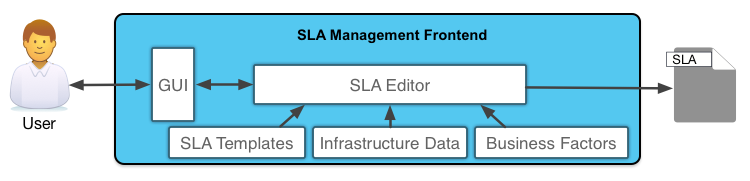
\includegraphics[width=5.3in]{chapters/chapter4/fig/Editor.PNG}
\caption{ASLAMaaS SLA Management Frontend Overview}
\label{fig_Editor}
\end{figure}

As described in Chapter \ref{SLA}, SLAs comprise the expected quality of service the provider has to deliver, which are recorded as the agreed service levels. The service levels include one or multiple KPIs, which describe in each case a specific QoS parameter and the associated metric to monitor. In order to allow users to choose the KPIs for their SLA contract self-reliant certain preconditions must be met. Since cloud architectures are constantly changing the available KPIs are provider dependent and must be pre-accepted beforehand. Therefore possible cloud relevant KPIs have been identified in Chapter \ref{Cloud KPIs} and must be selected initially by the provider.

Based on the provider accepted KPIs meaningful margins have to be calculated as basis for the SLA creation process. This is necessary because in this self-service approach the provider shall not have to engage in the process respectively negotiate with the consumer. The margins mark the boundaries in which a user can choose the service level. In order to provide only feasible conditions of which the user cam choose pre-calculations have to be made and pre-conditions have to be checked. For this purpose, various mathematical functions shall be examined for their suitability and expressiveness in order to integrate a suitable model.

Additionally the utilization, expected usage and performance data of the infrastructure shall be matched together with business concerns and the strategic focus of the provider to create a dynamic pricing model for the offered services and the corresponding SLAs. If, for example an infrastructure constantly delivers a response-time of below 170ms and only a few fluctuations of users are expected the reasoning model may set the lower margin for this KPI to 200ms or slightly above. Since it is common practice to make prices not directly on each possible service level, but to create pricing categories, such as low, medium, high or silver, gold platinum the delivered price model shall then create these pricing categories. This should enable a simpler management of the managed service levels and makes the gradation of customers easier for the system.
  
In order to autonomously conduct this process the SLA templates and the finished filled out SLAs used must be represented in a machine processable form. For this a machine readable agreement description language shall be used. The Adaptable Service Level Objective Agreement (A-SLO-A) model \cite{A-SLO-A}, which is based on the SLA* model, enables the use of dynamic and constant agreement alteration and therefore is will be used as the basis of the description of SLAs in ASLAMaaS.


\section{Prediction, Detection and Management of Service Levels} \label{SLA prediction}
%Mustererkennung / TODO REWRITE
%Anomaly Detection
%Detection of cloud resource misusage
%Prediction of cloud ressource usage
In order to guarantee the QoS of a provided service, it is necessary for particular things to be monitored. Firstly, the performance of the infrastructure must be monitored since dependencies arise in a multitenancy environment with shared resources. Secondly, the use of cloud services usually varies greatly and thus the need of resources fluctuates likewise. To cope with this changing needs and to achieve SLA  compliance the provided resources must be adjusted. If one could predict the usage of a service, looking ahead further than the infrastructure provisioning delay time, one could guarantee the QoS for that specific service. Therefore prediction and detection techniques should be 

To detect unforeseen events, the cloud components behavior is constantly monitored and analyzed. Therefore events from each of the CMS and monitoring agents are processed to enable anomalous behavior detection. 
To determine, which anomaly detection algorithms are suited best, an evaluation has to be done. The algorithms considered include machine learning approaches like neural networks or Markov models, statistical methods, outlier detection and some specialized algorithms \cite{Anomaly2}. %The main questions which need to be clarified by this research stage are:

The Plan part of the MAPE-K concept in this module creates the action plans fot the infrastructure, the CMS, the SLA Manager itself and additionally delivers adjustments directly back into the SLA Editor, where for example the margins could be readjusted to cope with the changes. Thus this the SLA templates and the corresponding KPI margins are always complaint with the actual performance of the cloud system. The action plans result in adaptation of the cloud infrastructure, like for example if the stated response-time inside a certain SLA tends to be broken the SLA manager can instruct the virtual network agent to re-route the traffic if the problem is network dependent. In case of this problem related to overloaded CPU or virtual instances the SLA Manager could start new instances or allocate more CPU cores.

The various methods to manage the QoS parameters have to be model individually and tested about their suitability. A sample for the regulation of the KPI response-time can be found at Frey et al. \cite{Fuzzy}. There scalable cloud services have been started and stopped based on a fuzzy control set. This and other similar control mechanisms enable the Execute part to adapt the infrastructure and the services so that SLA violations can be avoided and the QoS is guaranteed. Within both MAPE-K loops the Knowledge consist mainly of the historic data about the services, the SLAs and the cloud environment, which was measured continuously and expert knowledge in the form of best practices and empirical values as well as strategic business plans. %Techniken zur Prognose!!!!

\section{Evaluation of ASLAMaaS}
During and following the development of the ASLAMaaS prototype, the sub and complete system will be evaluated due to its performance and SLA compliance. For performance, experiments with increasing amounts of VMs (10,50,100,...) will be developed to show that the ASLAMaaS approach is scalable and can cope with rising dependencies. Further investigation will be done to clarify the following questions: How accurate is the generation of SLA templates based on the corresponding infrastructure data for the margins? How well is the prediction suited to foresee mutual influences of VM performance?  Can the QoS of the cloud services and the reliability be improved beyond business requirements ?

\section{Summary}
The proposed SLA management framework for cloud computing is a novel and robust specification, for supporting QoS and SLAs management in cloud infrastructures. It is designed to address the growing demand on QoS and performance guarantees arising from the increasing use of cloud computing by small and medium sized industries. Overall it aims to increase the reliability and transparency of cloud infrastructures, giving users the opportunity to manage their quality needs. At worst it is providing the same level of quality management currently found in cloud computing environments. At best, all cloud customers can benefit from it, by defining and changing on-demand the service levels for their cloud instances. SLA reports enable users to get a comprehensible knowledge about the status of their cloud instances at any time and enable continuous verifiable proof about the delivered services. Cloud providers will be able to estimate the potential performance of their infrastructures and based on that give customers service guarantees. Performance evaluation, prediction and behavior analysis is used to detect possible risks and intervene avert an SLA violations. The ASLAMaaS framework is based on concurrent autonomous management modules, which  evaluate the performance levels of cloud resources such as, cloud instances, storage, network and the cloud infrastructure as well as specific cloud services. This will improve the overall reliability and performance of cloud infrastructures.